\documentclass{article}
\usepackage[utf8]{inputenc}
\usepackage{amsmath}
\usepackage{mathtools}
\usepackage{float}
\usepackage[numbered, framed]{matlab-prettifier}
\usepackage[font=small]{caption}


\setlength{\abovecaptionskip}{3pt}
\setlength{\belowcaptionskip}{3pt}

\title{Control Theory 5}
\author{Kamil Kamaliev, Var b \\ k.kamaliev@innopolis.university }
\date{April 2020}

\lstset{
  style = Matlab-editor,
  basicstyle = \mlttfamily,
  escapechar = ",
  mlshowsectionrules = true,
}

\begin{filecontents*}{observability.m}
    A = [0 0 1 0; 0 0 0 1; 0 23.66 0 0; 0 37.6 0 0];
    B = [0; 0; 0.29; 0.33];
    C = [1 0 0 0; 0 1 0 0];
    D = [0; 0];
    sys = ss(A,B,C,D);
    
    Ob = obsv(A,C);
    unob = length(A)-rank(Ob);
    unob

\end{filecontents*}


\begin{filecontents*}{e.m}
    A = [0 0 1 0; 0 0 0 1; 0 23.66 0 0; 0 37.6 0 0];
    B = [0; 0; 0.29; 0.33];
    C = [1 0 0 0; 0 1 0 0];
    D = [0; 0];
    
    p = [-1 -0.5 -0.2 -0.1];
    
    K = place(A, B, p);
    L = place(A', C', p)';
    
    A_ = A - B * K - L * C;
    
    controlled_system = ss(A_, B, C, D);
    
    t = 0:0.1:10;
    u = sin(t);
    
    figure(1);
    subplot(121);
    step(controlled_system);
    title("Step response");
    subplot(122);
    y = lsim(controlled_system, u, t);
    plot(t, y);
    title("Sine response");
\end{filecontents*}


\begin{filecontents*}{eigenvals.m}

    A = [0 0 1 0; 0 0 0 1; 0 23.66 0 0; 0 37.6 0 0];
    B = [0; 0; 0.29; 0.33];
    C = [1 0 0 0; 0 1 0 0];
    D = [0; 0];
    sys = ss(A,B,C,D);
    
    eig(A)
\end{filecontents*}

\begin{filecontents*}{lqr.m}

    A = [0 0 1 0; 0 0 0 1; 0 23.66 0 0; 0 37.6 0 0];
    B = [0; 0; 0.29; 0.33];
    C = [1 0 0 0; 0 1 0 0];
    D = [0; 0];
    
    N = [0 0; 0 0; 0 0; 0 0];
    Q = [1 0 0 0; 0 1 0 0; 0 0 1 0; 0 0 0 1];
    R = [1];
    
    [K,S,e] = lqr(transpose(A), transpose(C), Q, R, N);
    L = transpose(K);
    L
\end{filecontents*}

\begin{filecontents*}{pole.m}

    A = [0 0 1 0; 0 0 0 1; 0 23.66 0 0; 0 37.6 0 0];
    B = [0; 0; 0.29; 0.33];
    C = [1 0 0 0; 0 1 0 0];
    D = [0; 0];
    
    p = [-1 -0.5 -0.2 -0.1]
    
    L = place(A', C', p)';
    L
\end{filecontents*}

\begin{filecontents*}{fb_cont.m}

    A = [0 0 1 0; 0 0 0 1; 0 23.66 0 0; 0 37.6 0 0];
    B = [0; 0; 0.29; 0.33];
    C = [1 0 0 0; 0 1 0 0];
    D = [0; 0];
    
    p = [-1 -0.5 -0.2 -0.1]
    
    K = place(A, B, p);
    K
\end{filecontents*}

\begin{filecontents*}{awgn_output.m}
    A = [0 0 1 0; 0 0 0 1; 0 23.66 0 0; 0 37.6 0 0];
    B = [0; 0; 0.29; 0.33];
    C = [1 0 0 0; 0 1 0 0];
    
    p = [-1 -0.5 -0.2 -0.1];
    
    K = place(A, B, p);
    L = place(A', C', p)';
    
    A_ = A - B * K - L * C;
    t = 0:0.01:10;
    size(t)
    
    controlled_system = ss(A_, -1 * L, C, [1 0; 0 1]);
    
    
    u = zeros(2, 1001);
    u_noise = awgn(u, 10);
    z0 = [-0.2, 0, 0.1, 0.03];
    
    figure(1);
    subplot(121);
    [y, t, z] = lsim(controlled_system, u, t, z0);
    z
    plot(t, z(:, 1:2));
    title('Without noise');
    subplot(122); 
    [y, t, z] = lsim(controlled_system, u_noise, t, z0);
    plot(t, z(:, 1:2));
    title('With AWGN');
\end{filecontents*}

\begin{filecontents*}{awgn_state.m}
    A = [0 0 1 0; 0 0 0 1; 0 23.66 0 0; 0 37.6 0 0];
    B = [0; 0; 0.29; 0.33];
    C = [1 0 0 0; 0 1 0 0];
    
    p = [-1 -0.5 -0.2 -0.1];
    
    K = place(A, B, p);
    L = place(A', C', p)';
    
    A_ = A - B * K - L * C;
    t = 0:0.01:10;
    size(t)
    
    u = zeros(1, 1001);
    u_noise = awgn(u, 10);
    z0 = [-0.2, 0, 0.1, 0.03];
    
    figure(1);
    controlled_system = ss(A_, [1; 1; 1; 1], C, [0; 0]);
    subplot(121);
    [y, t, z] = lsim(controlled_system, u, t, z0);
    plot(t, z(:, 1:2));
    title('Without noise');
    subplot(122);
    [y, t, z] = lsim(controlled_system, u_noise, t, z0);
    plot(t, z(:, 1:2));
    title('With AWGN');
\end{filecontents*}

\begin{filecontents*}{kalman.m}
    A = [0 0 1 0; 0 0 0 1; 0 23.66 0 0; 0 37.6 0 0];
    B = [0; 0; 0.29; 0.33];
    C = [1 0 0 0; 0 1 0 0];
    D = [0; 0];
    
    p = [-1 -0.5 -0.2 -0.1];
        
    K = place(A, B, p);
    L = place(A', C', p)';
        
    new_A = A - B*K - L*C;
    
    B_ = [B [0; 0; 0; 0] [1; 1; 1; 1]];
    D_ = [D [1; 1] [0; 0]];
    sys = ss(new_A, B_, C, D_);
    
    t = 0:0.01:10;
    u = sin(t);
    v = randn(1, length(t));
    w = randn(1, length(t));
    ua = [u; v; w];
    
    Q = 1;
    R = [1 0; 0 1];
    
    [kest, L, P] = kalman(sys, Q, R);
    kest = kest(1, :);
    
    s = parallel(sys, kest, 1, 1, [], []);
    SimModel = feedback(s, 1, 4, 2, 1);
    SimModel = SimModel([1 3], [1 2 3]);
    [out, x] = lsim(SimModel, ua, t);
    y = out(:, 1);
    yf = out(:, 2);
    
    figure(1);
    plot(t, y, 'r', t, yf, 'b');
    hold on
    [yn, x] = lsim(sys, ua, t);
    plot(t, yn(:, 1), '--g');
    title('Kalman Filter');
    legend('True Response', 'Kalman Filter', 'Noisy System');
\end{filecontents*}

\begin{document}

\maketitle

 $$
        \left\{ \begin{array}{ll} 
            (M+m)x^{\prime\prime}-mlcos(\theta)\theta^{\prime\prime}+mlsin(\theta)\theta^{\prime^2} = F\\
            -cos(\theta)x^{\prime\prime}+l\theta^{\prime\prime}-gsin(\theta) = 0
        \end{array} \right.
$$

The linearization of the system was performed using the tools from the previous homework with values $M = 3.4, \ m = 8.2, \ l = 0.89:$

         $$
        \left\{ \begin{array}{ll} 
            \delta z'= A \delta z + B \delta u\\
            \delta y = C \delta z
        \end{array} \right.
        $$
        
where

$$
A = \begin{bmatrix}
0 & 0 & 1 & 0 \\
0 & 0 & 0 & 1 \\
0 & 23.66 & 0 & 0 \\
0 & 37.6 & 0 & 0
\end{bmatrix}, \ 
B = \begin{bmatrix}
0 \\
0 \\
0.29 \\
0.33
\end{bmatrix}, \ 
C = \begin{bmatrix}
1 & 0 & 0 & 0 \\
0 & 1 & 0 & 0 \\
\end{bmatrix} ,
$$

\paragraph{A. Possibility to design state observer}

\leavevmode

\noindent
The required check was made by constructing observability matrix with the following Matlab Code:
 
\lstinputlisting[caption={Checking the observability of the system}]{observability.m}

\noindent
unob shows the number of unobservable states.

\noindent
In my case, it's equal to 0.

\newpage

\paragraph{B. Stability of error dynamics}
\leavevmode

\noindent
We have a system with dynamics $z' = Az + Bu $. Thus, the open loop state observer is $\overline{z}' = A\overline{z} + Bu$. 

\noindent
From this, we may derive the error: $e = z - \overline{z}$. And after subtracting $z'$ from $z$, we obtain: $e' = Ae$.

\noindent
To check the stability, one may find the eigenvalues of $A$. This was done by the following Matlab code:

\lstinputlisting[caption={Obtaining eigenvals of matrix A}]{eigenvals.m}

\noindent
the result is : $ 
\begin{bmatrix}
0 \\
0 \\
6.1319 \\
-6.1319
\end{bmatrix}
$

\vskip

\noindent
As we can see, 1 eigenvalue is positive making the error dynamics unstable.


\paragraph{C. Luenberger observer}
\leavevmode

\noindent
We have a system 
$$
        \left\{ \begin{array}{ll} 
            z' = Az + Bu\\
            y = Cz
        \end{array} \right.
$$

\noindent
and the following observer $\overline{z}' = A\overline{z} + Bu + L(y - \overline{y})$. After deriving error $e = \overline{z} - z$ and subtracting $z'$ from $\overline{z}'$ we obtain:

$$e' = (A - LC)e$$

\noindent
We need to find such $L$ that makes the matrix $A - LC$ negative definite. This is the same as finding such $L$ that makes matrix $A^T - C^TL^T$

\noindent
\textbf{LQR Way}
For weight matrices we may take Identity matrices. The L is found by the following Matlab code:
\lstinputlisting[caption={LQR Method}]{lqr.m}

\noindent
The result is L = 
$
\begin{bmatrix}
4.1118 & 4.7048 \\
4.7048 & 10.0914 \\
19.0208 & 37.7669 \\
 29.0557 & 61.4856
\end{bmatrix}
$

\noindent
\textbf{Pole Placement Way}
\leavevmode

\noindent
For the error to be stable, we take negative numbers for poles. The L is found by the following Matlab code:
\lstinputlisting[caption={Pole Placement Method}]{pole.m}

\noindent
The result is L = 
$
\begin{bmatrix}
0.3 & 0 \\
0 & 1.5 \\
0.02 & 23.66 \\
0 & 38.1
\end{bmatrix}
$

\paragraph{D. State Feedback Controller}
\leavevmode

\noindent
We have the following system:
$$
        \left\{ \begin{array}{ll} 
            z' = Az + Bu\\
            u = -Kz
        \end{array} \right.
$$

\noindent
From which we obtain: $z' = (A - BK)u$.

\noindent
Now, we need to find such $K$ that makes $A - BK$ negative definite. This may be done using the pole placement method just like in the previous exercise by the following code:

\lstinputlisting[caption={Finding K}]{fb_cont.m}

The result is K = 
$
\begin{bmatrix}
-0.0032 & 116.8816 &   -0.0581 & 5.5056 
\end{bmatrix}
$

\paragraph{E. Simulation}
\leavevmode

\noindent
After adding control and observer, we obtain:  $z' = (A - BK - LC)z$. 

\lstinputlisting[caption={Simulation}]{e.m}

\begin{figure}[hbt!]
        \centering
        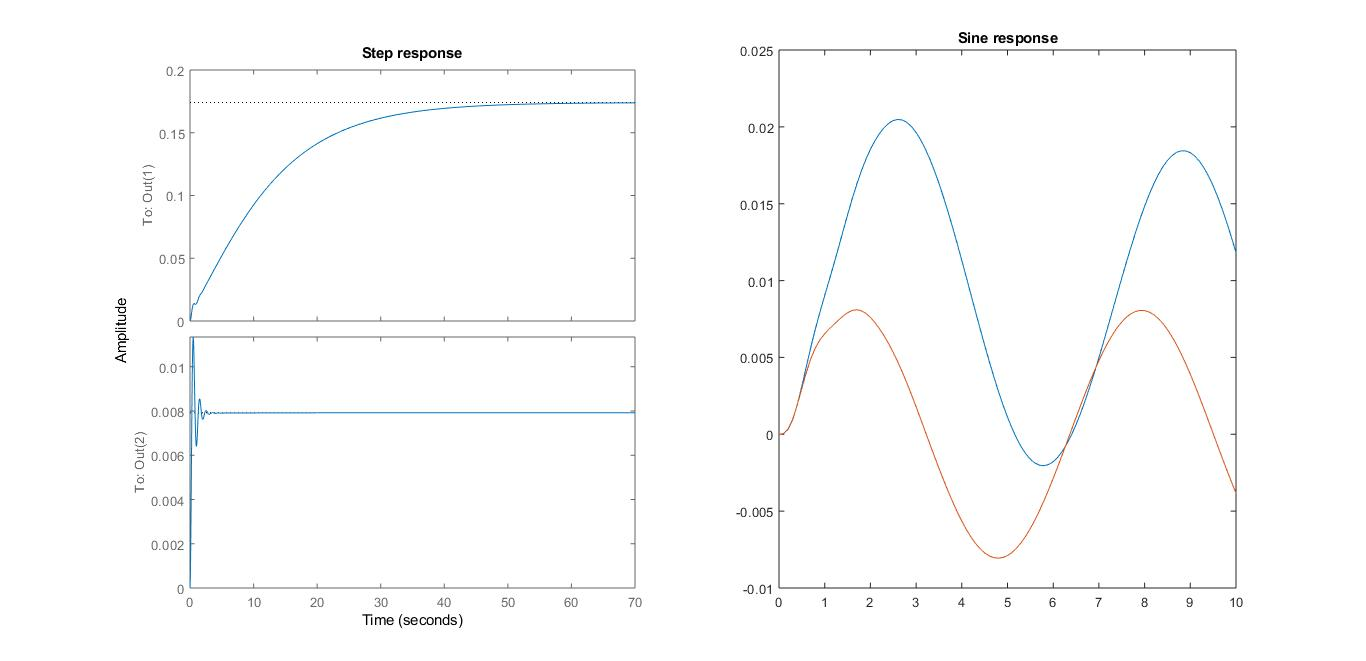
\includegraphics[scale=0.2]{e.jpg}
        \caption{Simulation}
\end{figure}

As we can see in Figure 1 (which for some reason went to task F), the system is stable, observer works quite good but the scaling is not quite right.

\vskip
\paragraph{F. AWGN in the output}
\leavevmode

\noindent
After adding controller, observer to the system and noise to the output, we obtain the following system:
    $$
    \left\{ \begin{array}{ll} 
        \delta z^\prime = A\_ \cdot \delta z + B\_ \cdot u\\
        \delta y = C \cdot \delta z + u
    \end{array} \right.
    $$

\noindent
where $A\_ =  (A - BK - LC) $, $B\_ = -L$ and $u = v$

\noindent
After these substitution, we can represent our dynamics in SS: 
\lstinputlisting[caption={AWGN in output}]{awgn_output.m}

\noindent
Which gives the following output:
\noindent
\begin{figure}[hbt!]
        \centering
        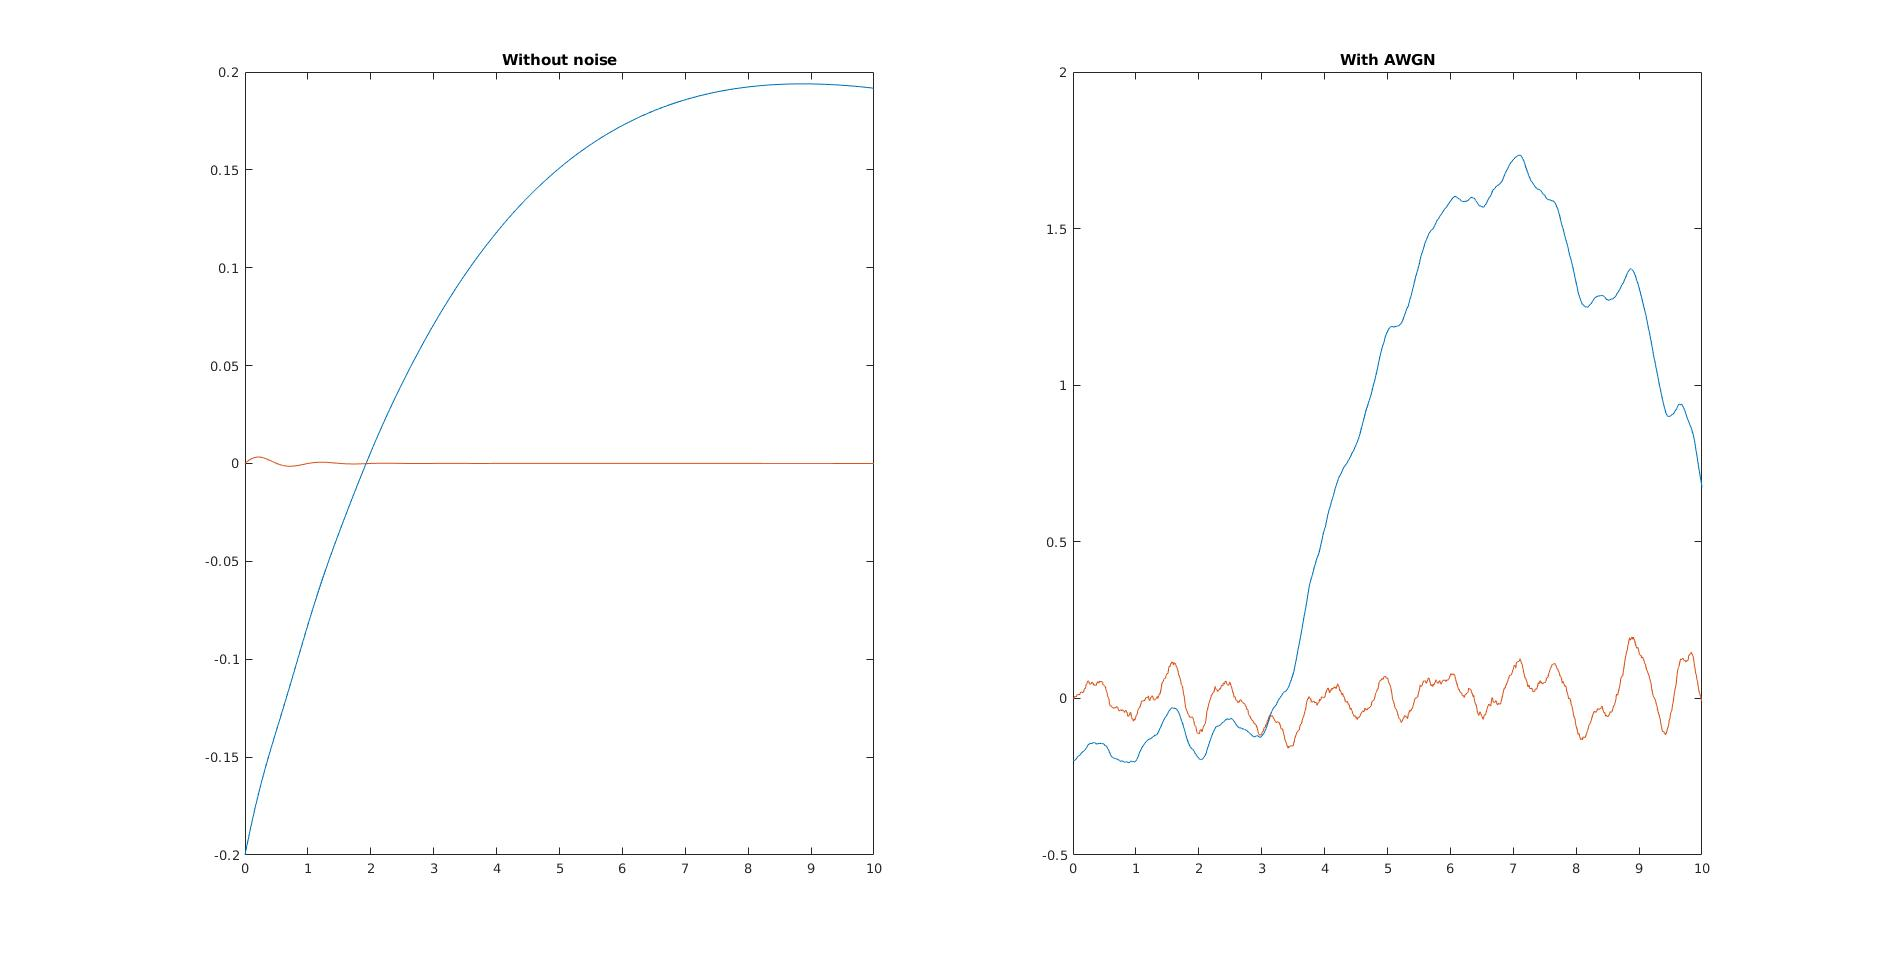
\includegraphics[scale=0.2]{task_f.jpg}
        \caption{Graphs of $x$ and $\theta$}
\end{figure}

\noindent
As Luenberger observer works with systems with no noise in the output, adding a noise (which is each time multiplied by $L$) to the output makes everything very terrible.

\paragraph{G. AWGN in the state}
\leavevmode

\noindent
After adding noise to the state dynamics, we obtain the following system:
$$
    \left\{ \begin{array}{ll} 
        \delta z^\prime = A\_ \cdot \delta z + \cdot u\\
        \delta y = C \cdot \delta z
    \end{array} \right.
    $$

\noindent
where $A\_ =  (A - BK - LC) $ and $u = w$


\noindent
After these substitution, we can represent our dynamics in SS: 
\lstinputlisting[caption={AWGN in output}]{awgn_state.m}

\noindent
Which gives the following output:

\noindent
\begin{figure}[hbt!]
        \centering
        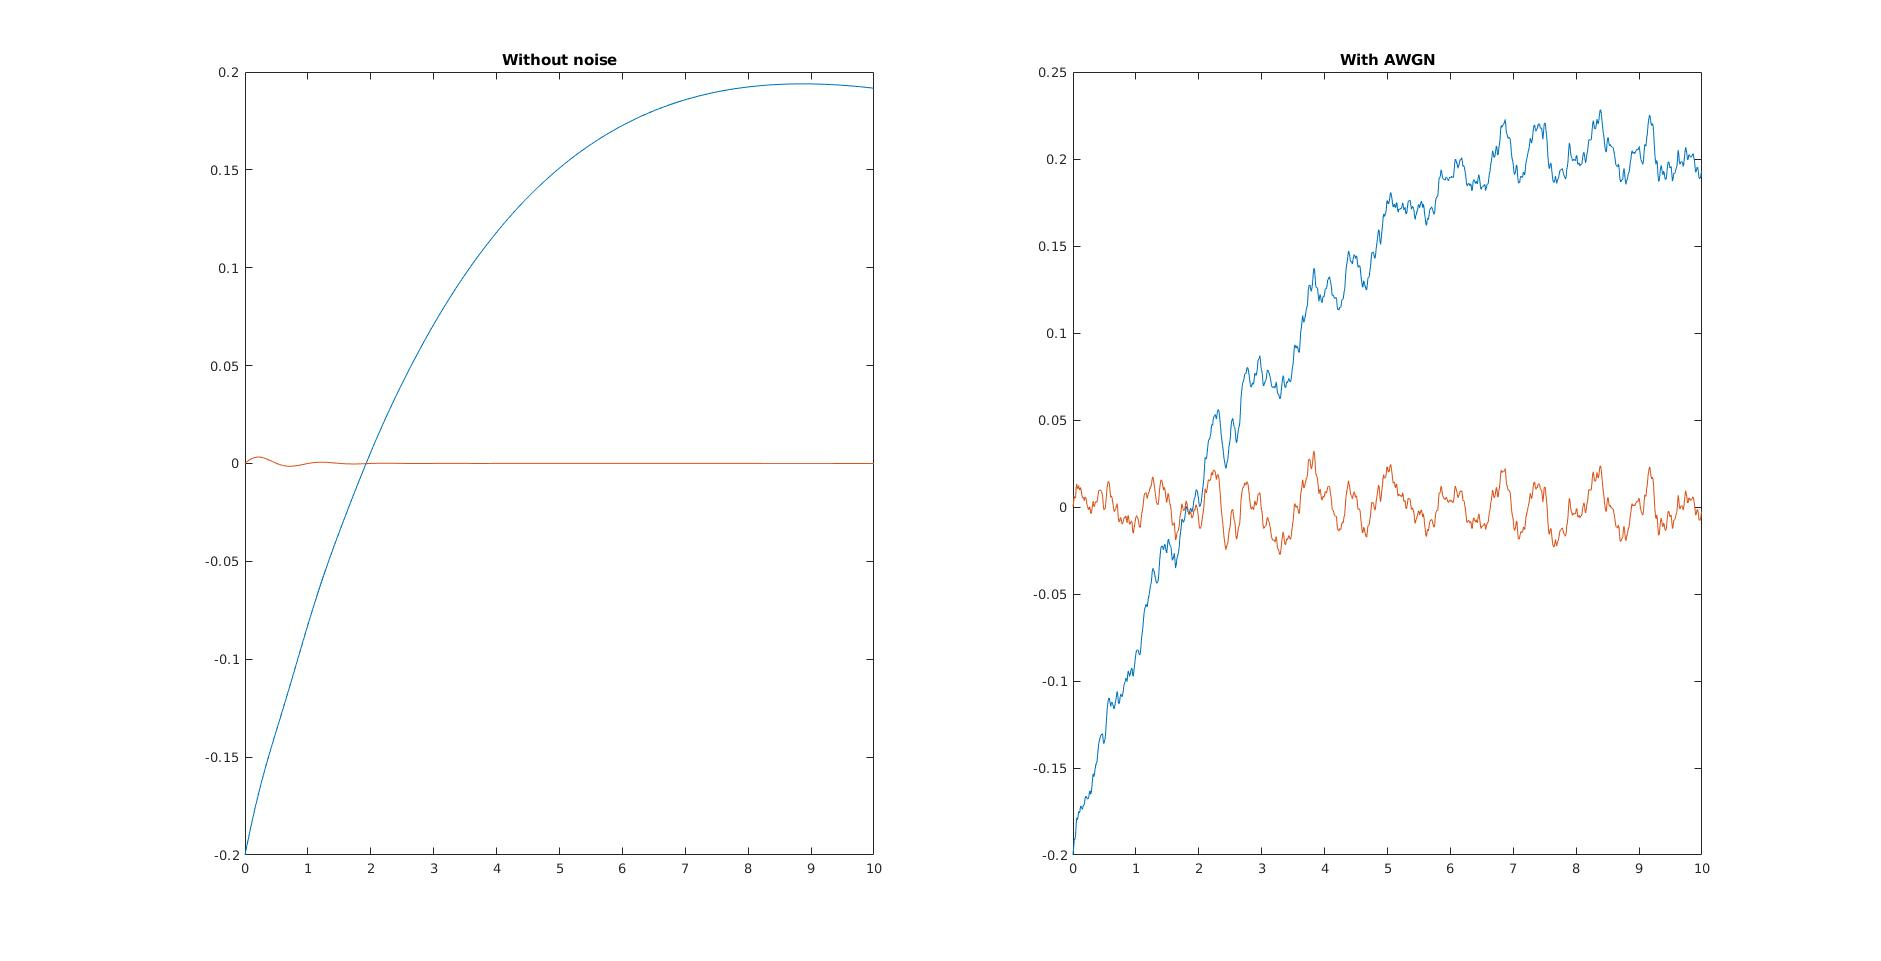
\includegraphics[scale=0.2]{task_g.jpg}
        \caption{Graphs of $x$ and $\theta$}
\end{figure}

\noindent
As we can see, adding noise to the state dynamics didn't make every very terrible as last time. This is because Gaussian noise is taken from a standard normal distribution centered at 0. 

\noindent
Due to the noise, absolute stability is lost. Nevertheless, seems like after some time the system will go into some kind of "borders", within which it will fluctuate.


\paragraph{H. Kalman Filter}
\leavevmode

\noindent
I decided to use MatLab library
\lstinputlisting[caption={Kalman}]{kalman.m}

\begin{figure}[hbt!]
        \centering
        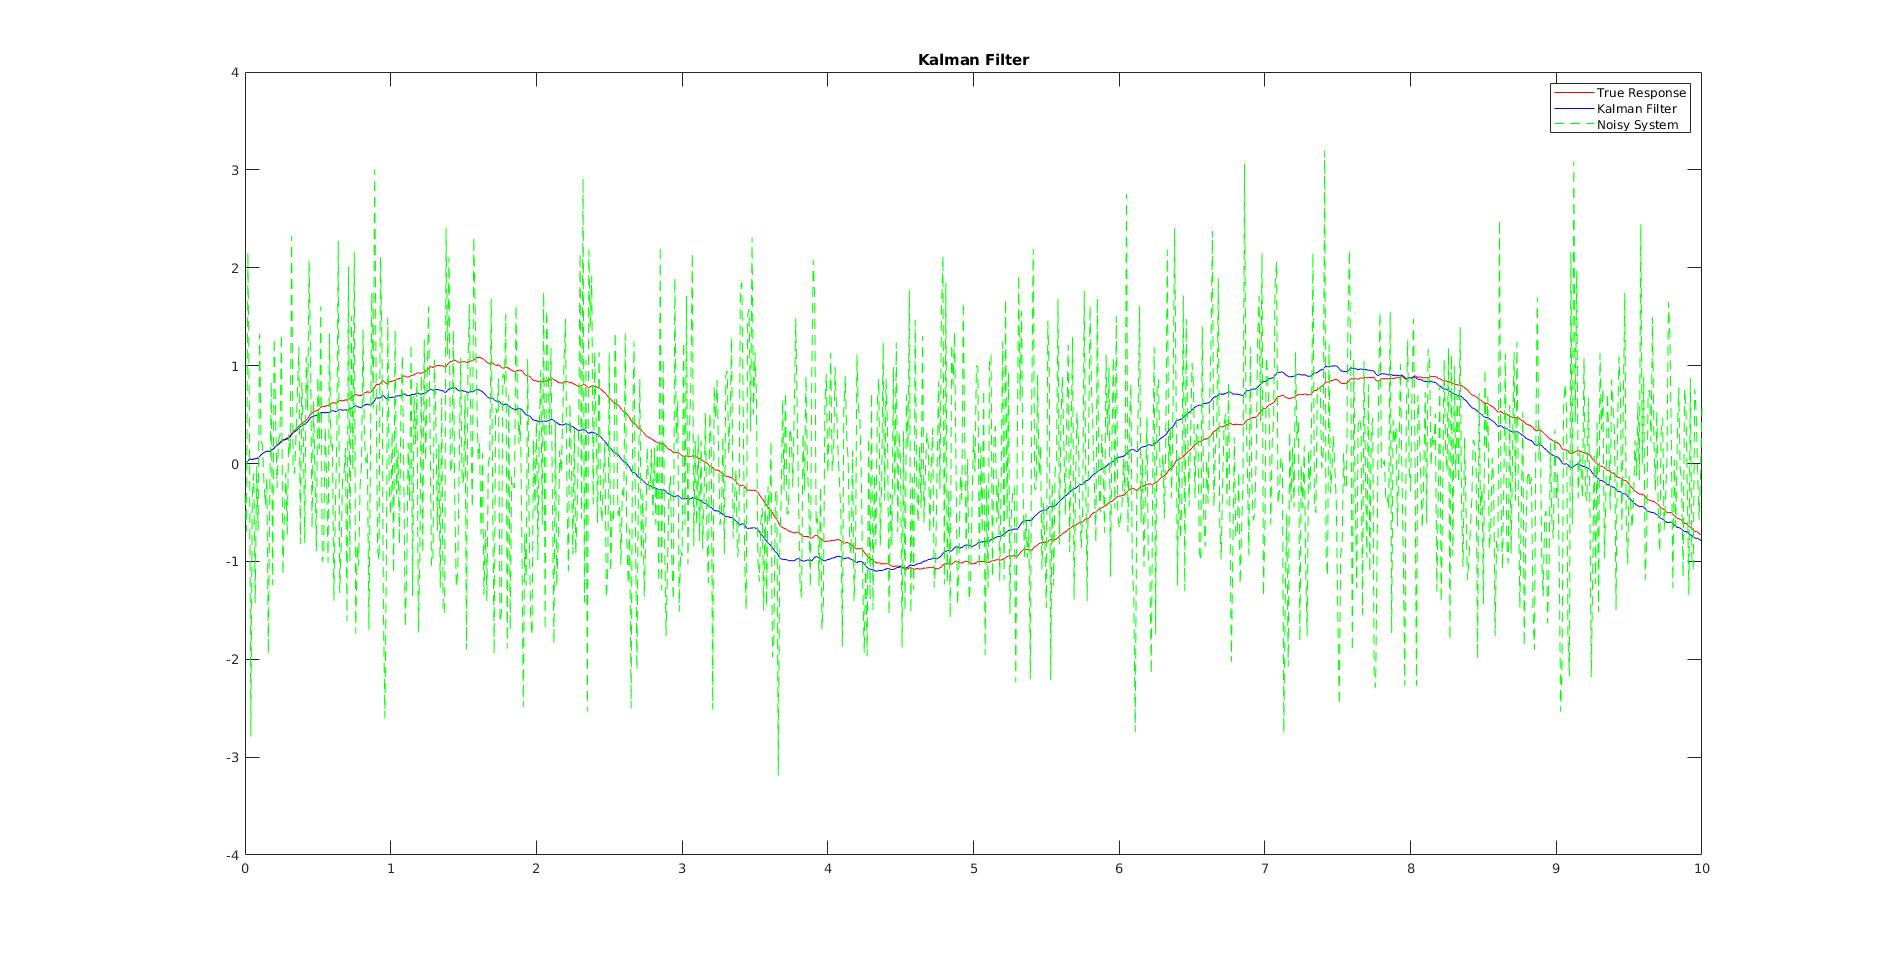
\includegraphics[scale=0.2]{kalman.jpg}
        \caption{Kalman}
\end{figure}

\end{document}
